\documentclass{article}
\usepackage[table,xcdraw]{xcolor} 
\usepackage{tcolorbox}
\usepackage{lipsum} 
\usepackage{array} 
\usepackage{tikz} 
\usetikzlibrary{shapes} 
\usepackage{pgffor} 
\usepackage{multicol} 
\usepackage{ifthen}


\newcounter{kulcsgondolat}
\setcounter{kulcsgondolat}{0}

\newcolumntype{Z}[2]{>{\columncolor{#1}\color{#2}} p{3cm}}


\newtcolorbox{sajatkornyezet}[2][]{
	colback=white, 
	colframe=black, 
	boxrule=0.5mm, 
	width=0.8\textwidth, 
	center title,
	title={#2},
	before upper={\vspace{1em}\noindent\rule{\textwidth}{0.4pt}\vspace{1em}},
	after upper={\vspace{1em}\noindent\rule{\textwidth}{0.4pt}\vspace{1em}}
}

\begin{document}
	
	
	\section{Első szakasz}
	\begin{sajatkornyezet}[Kulcsgondolatok]
		\gondolat\lipsum[1]
		\gondolat\lipsum[2]
	\end{sajatkornyezet}
	
	\section{Második szakasz}
	\setcounter{kulcsgondolat}{0} 
	\begin{sajatkornyezet}[Kulcsgondolatok]
		\gondolat\lipsum[3]
		\gondolat\lipsum[4]
	\end{sajatkornyezet}
	
	
	\begin{table}[ht]
		\centering
		\begin{tabular}{|Z{white}{black}|Z{gray!20}{black}|Z{white}{black}|}
			\hline
			\textbf{Osztály} & \textbf{Tantárgy} & \textbf{Érdemjegy} \\
			\hline
			\rowcolor{gray!20}\textbf{1} & Matematika & 5 \\
			\rowcolor{white}\textbf{2} & Fizika & 4 \\
			\rowcolor{gray!20}\textbf{3} & Kémia & 3 \\
			\rowcolor{white}\textbf{4} & Biológia & 5 \\
			\rowcolor{gray!20}\textbf{5} & Történelem & 4 \\
			\hline
		\end{tabular}
		\caption{Zebra táblázat példa}
		\label{tab:zebra}
	\end{table}
	
	
	\section{TikZ ábra}
	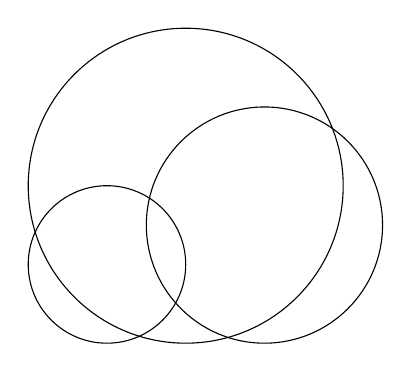
\begin{tikzpicture}
		
		\foreach \x/\y/\r in {1/1/1, 2/2/2, 3/1.5} {
			\draw (\x, \y) circle (\r);
		}
	\end{tikzpicture}

	
	\section{Számok kiírása 1-től 60-ig}
	\begin{multicols}{3}
		\newcounter{counter}
		\setcounter{counter}{1} 

		\whiledo{\value{counter} < 61}{
			
			\def\text{} 
			\ifnum\value{counter} \mod 3=0
				\edef\text{\text cikk}
			\fi
			\ifnum\value{counter} \mod 5=0
				\edef\text{\text cakk}
			\fi
			
			\thecounter \text\par
			\stepcounter{counter} 
		}
	\end{multicols}

\end{document}
